\section{Electronics}

In this section the design choices of the power supply and the photo diode circuit is described.
These are implemented as two separate boards as their functionality does not cross.

\subsection{Power supply}
One of the tasks of the project was to create a power supply for the FPGA board and the external components. 
This supply should take a 15 V signal and divide it into 3 different voltage levels which can be seen in table \ref{tab::power_req}. 
The power supplys is soldered on a PCB made using Eagle, a CAD program for circuit design. 
The schematic of the board can be seen on figure \ref{fig::sch_power}.
\subsubsection{Regulators}
\begin{wraptable}{r}{7cm}
 \vspace{5 pt}
 \begin{tabular}{cccc}
  Voltage & Current & Tolerance      & Efficiency \\ \toprule
  12 V    & 1.0 A   & -              & -          \\
  6 V     & 1.5 A   & -              & -          \\
  5 V     & 0.5 A   & $\pm\ 1.5 \%$  & 80\%       \\
  \bottomrule
 \end{tabular}
\caption{Voltage and current requirements for the power supply.}
\label{tab::power_req}
 \vspace{5 pt}
\end{wraptable}
The 5 V supply, driving the FPGA, has a requirement to the efficiency which means a switching regulator must be used for this task. 
For the switching regulator a LM2574N-5.0 was chosen as it provides a 0.5A, 5.0V supply.
According to the datasheet, the typical efficiency is 77\% \cite{ds:LM2574N}. 
The switching regulator is the best available to this project so this is overlooked.

The specified tolerance is 4\% which means the tolerance is worse than required. Further testing is required to see if the configuration is good enough for the application\cite[p. 1]{ds:LM2574N}.
The power supply is tested under load in section \ref{sec:test_pwr_supply}.

The schematic was designed following the typical application guidelines in the datasheet.
The diode was selected as 1N5817\cite[p. 17]{ds:LM2574N}. 
The $C_{out}$ capacitor was chosen to be $330\mu f$ to minimize ripple voltage\cite[p. 19]{ds:LM2574N}.

Given the input voltage of 15 V and the max current drawn, $0.5 A$, the value of the inductor should be 330 $\mu H$\cite[p. 14]{ds:LM2574N}.

The schematic for the 5 V supply can be seen in figure \ref{fig::sch_power_5V}.

There is no requirements to the efficiency of the 6 and 12 V supplys so a linear regulator is used.
The maximum current in the 6 V supply is 1.5 A, which means a bigger diode is needed.
For this a 1N5408 is chosen, which can deliver an average 3.0 A forward current\cite[p. 1]{ds:1N5408}.

The capacitors are there to eliminate voltage spikes from the load. A capacitance of $0.1 \mu F$ is chosen based on the recommendations\cite[p. 702]{book:prac_ele}.
The schematics of the 6 and 12 V supplys can be seen in figure \ref{fig::sch_power_6V} and \ref{fig::sch_power_12V}.

\begin{figure}[H] %left, bot, right, top
\centering
\begin{subfigure}{0.3\linewidth}
\centering
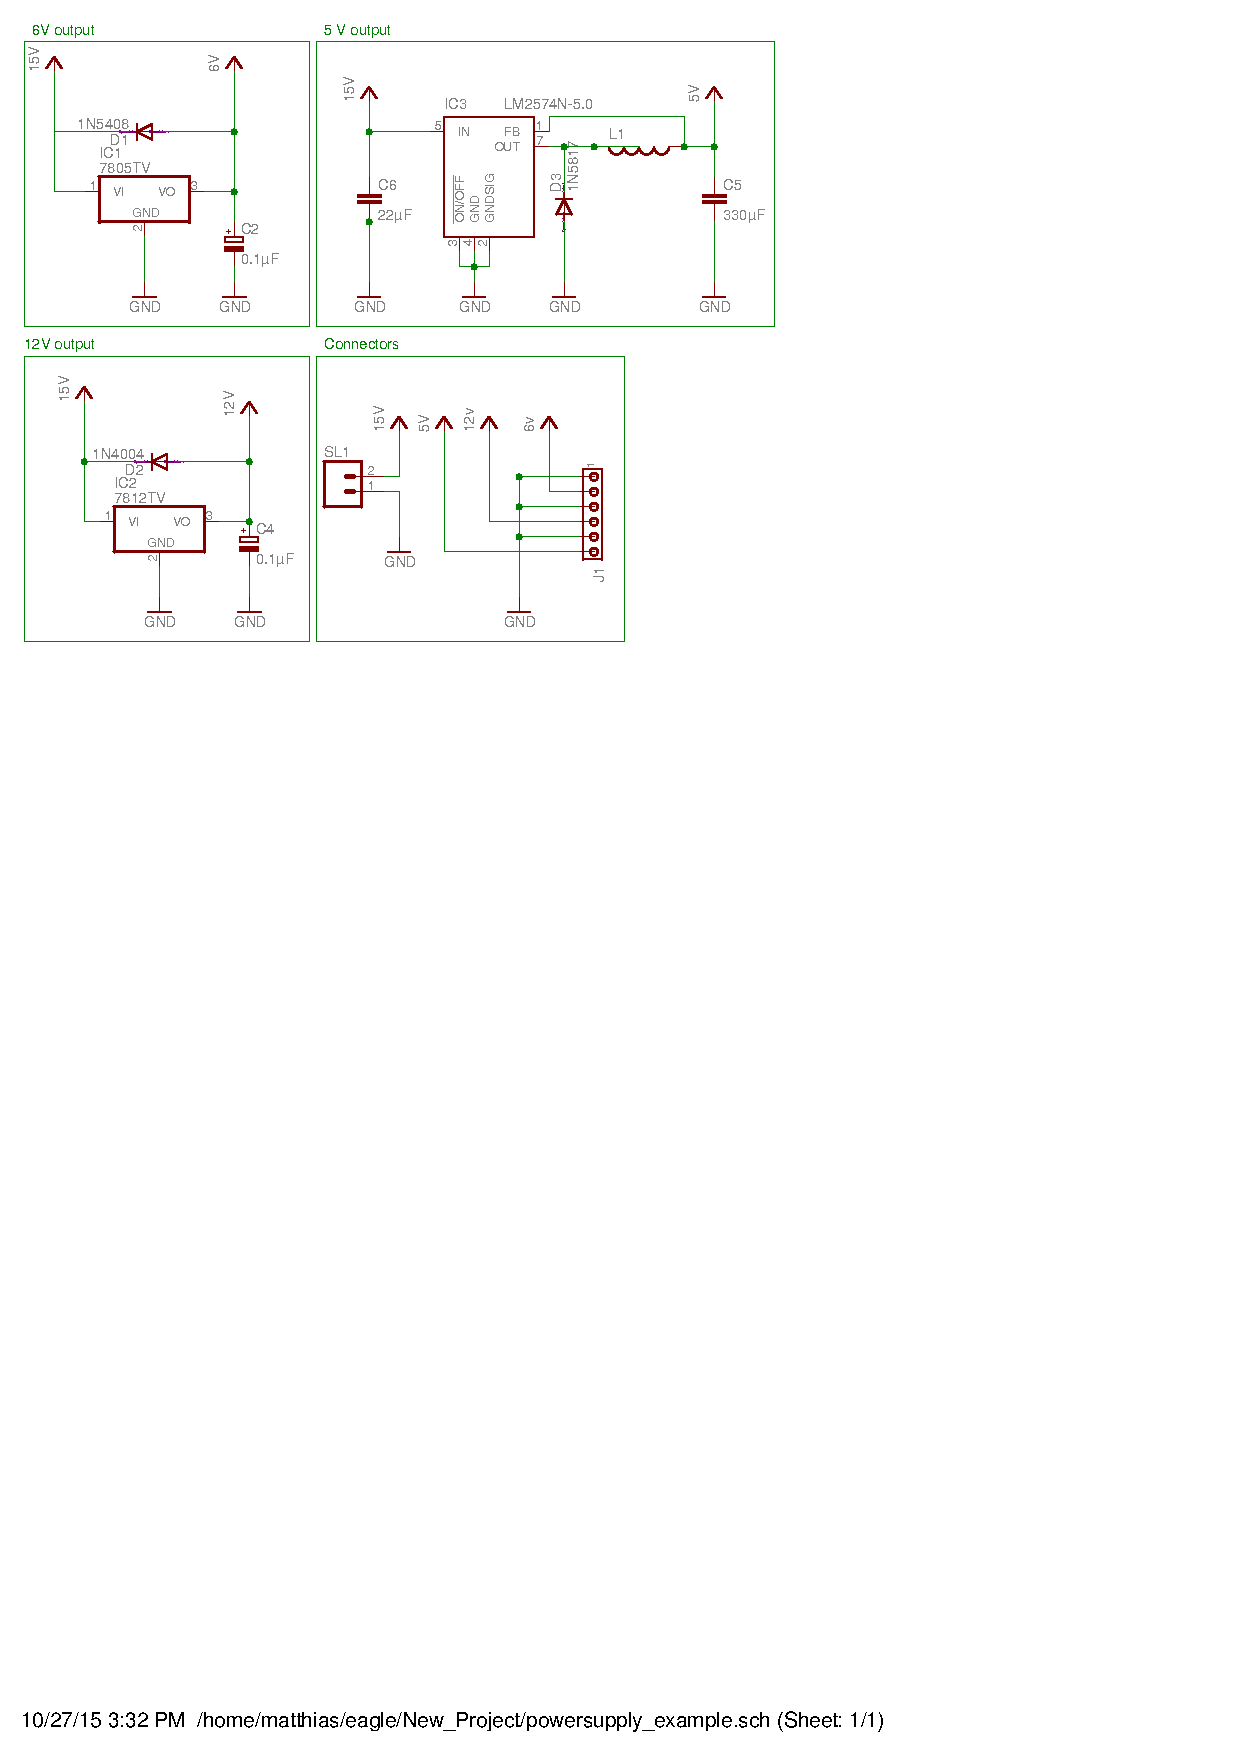
\includegraphics[scale=0.8,trim={0 24cm 15.7cm 0.6cm},clip]{img/powersupply.pdf}
\caption{6 V supply.}
\label{fig::sch_power_6V}
\end{subfigure}
\begin{subfigure}{0.5\linewidth}
\centering
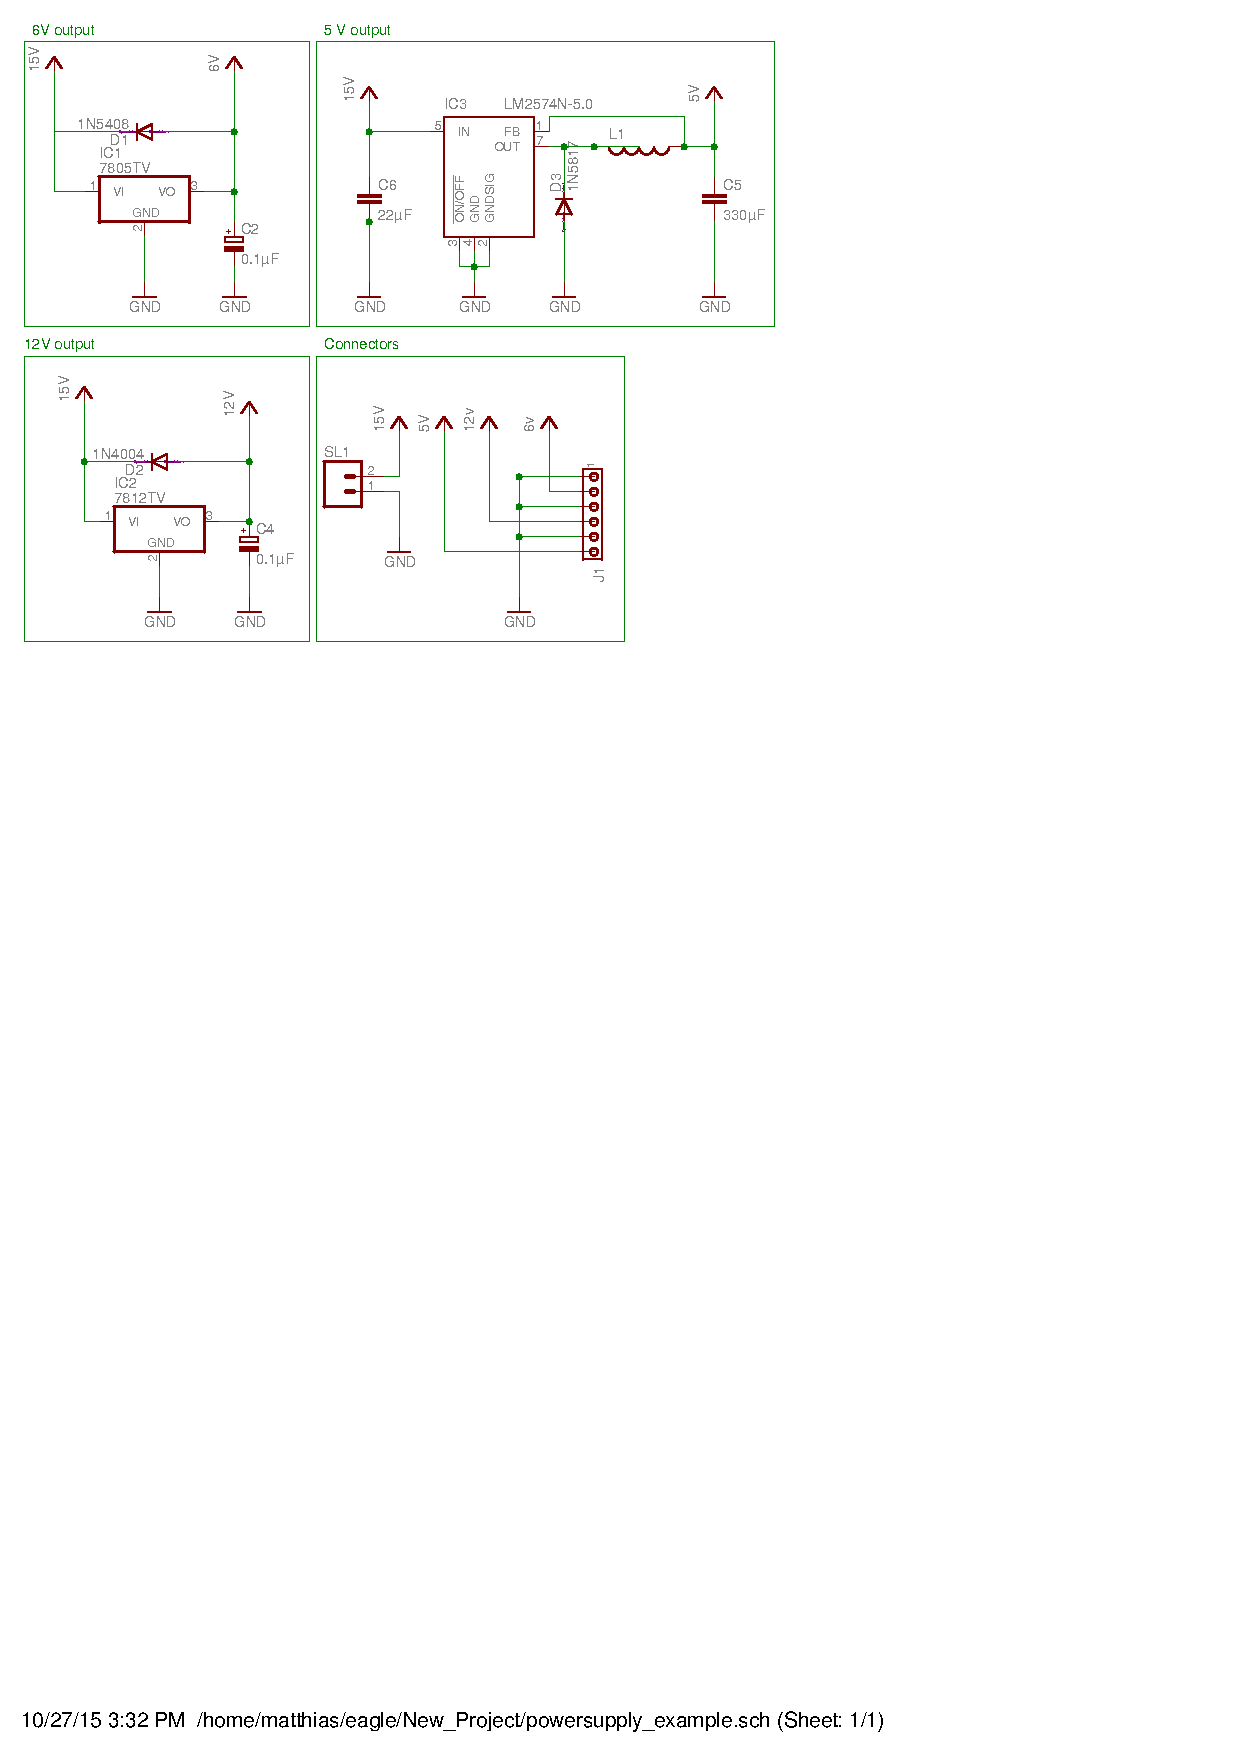
\includegraphics[scale=0.8,trim={5.3cm 24cm 7.8cm 0.6cm},clip]{img/powersupply.pdf}
\caption{5 V supply.}
\label{fig::sch_power_5V}
\end{subfigure}

\begin{subfigure}{0.3\linewidth}
\centering
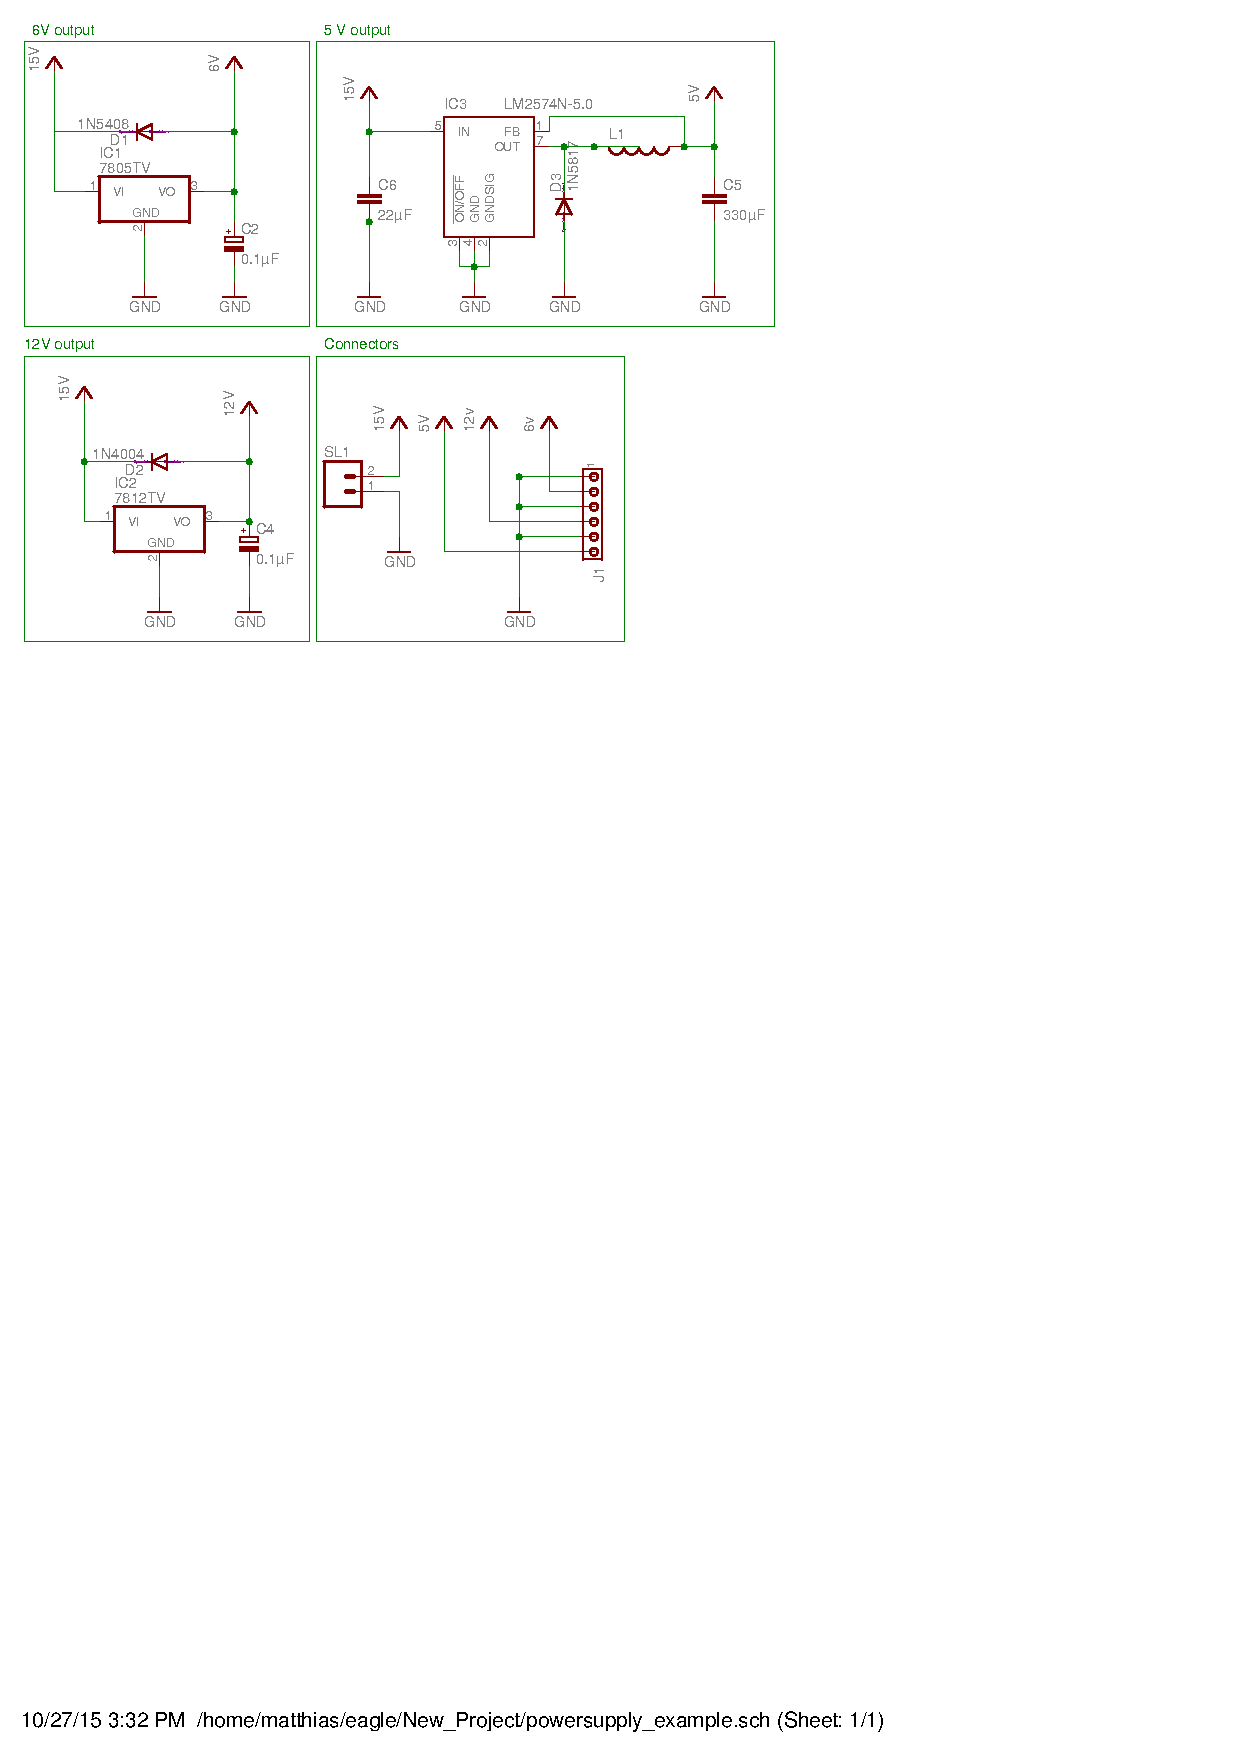
\includegraphics[scale=0.8,trim={0 18.5cm 15.7cm 6.0cm},clip]{img/powersupply.pdf}
\caption{12 V supply.}
\label{fig::sch_power_12V}
\end{subfigure}
\begin{subfigure}{0.5\linewidth}
\centering
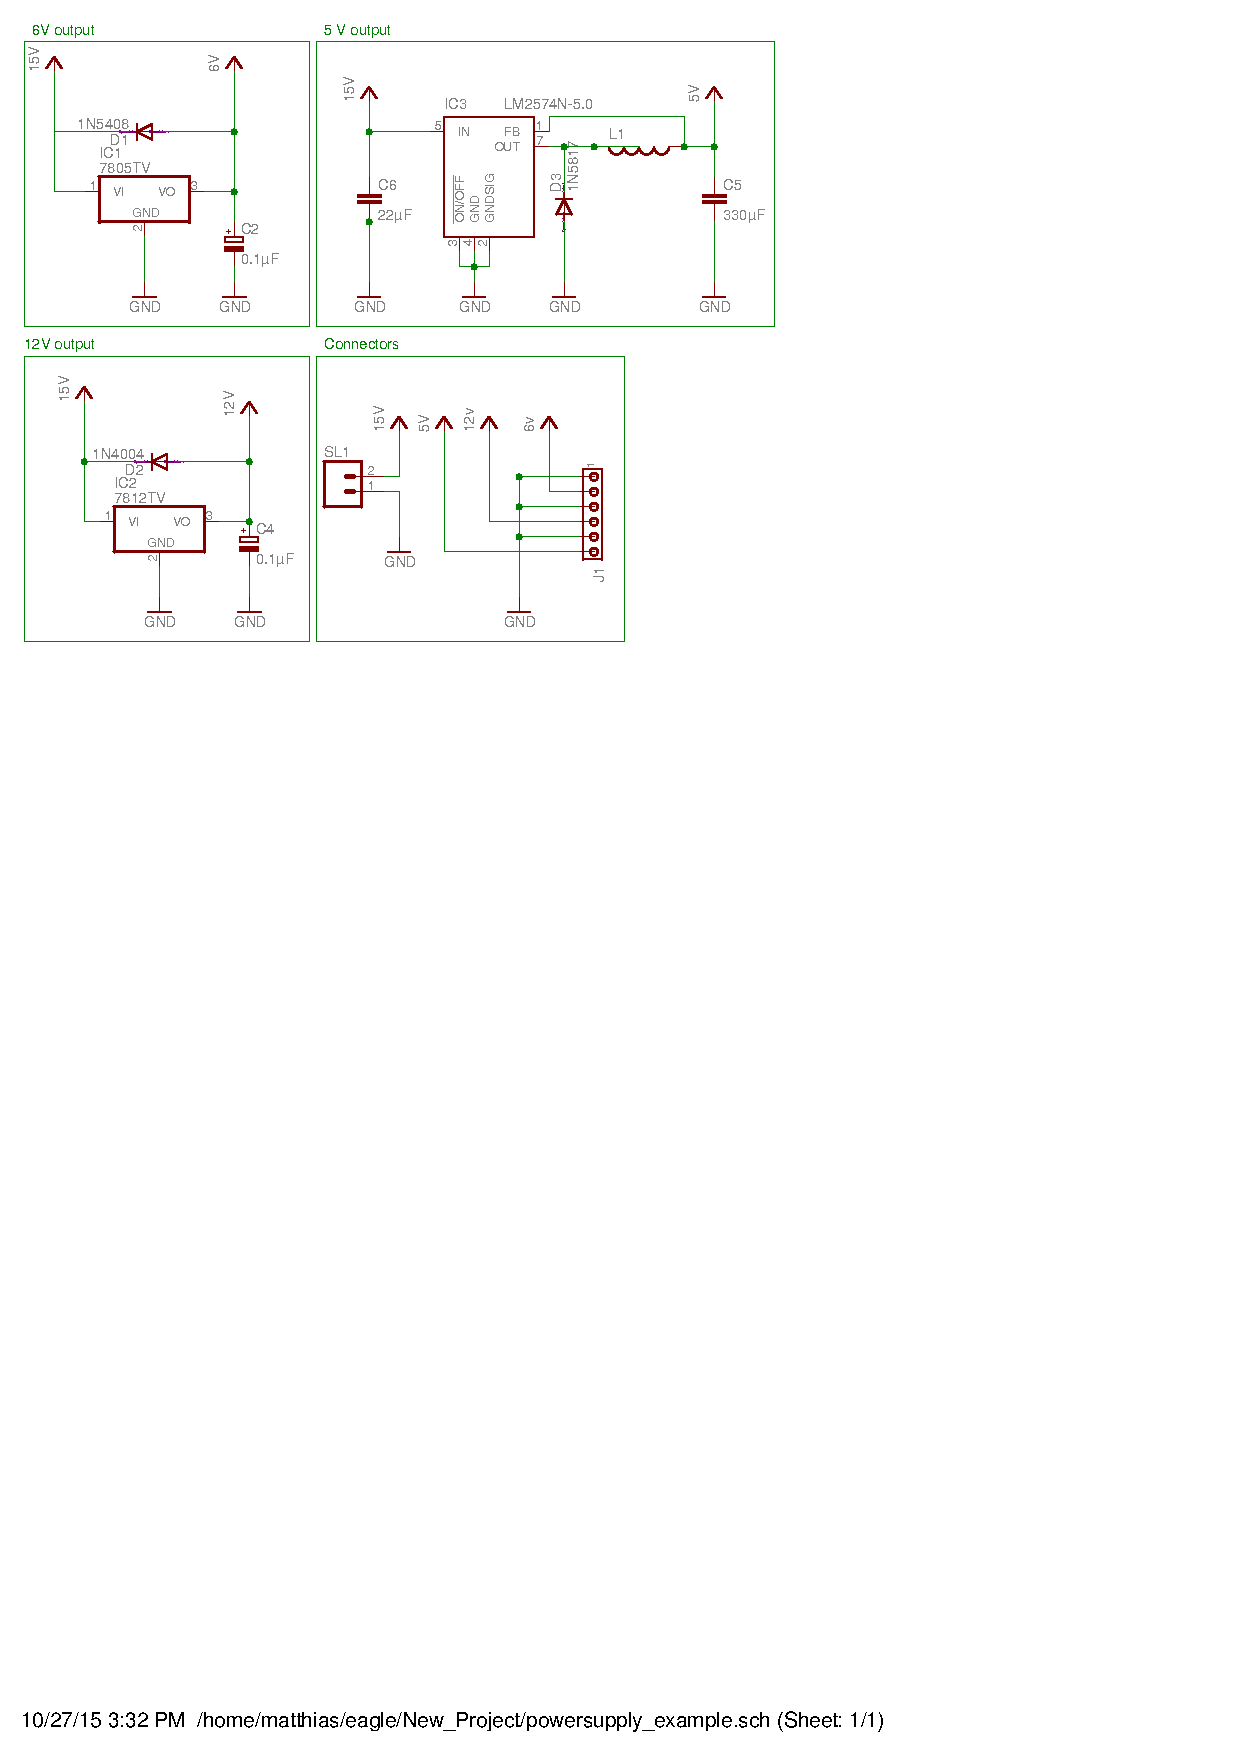
\includegraphics[scale=0.8,trim={5.3cm 18.5cm 10.4cm 6.0cm},clip]{img/powersupply.pdf}
\caption{Breakout pins.}
\label{fig::sch_power_pins}
\end{subfigure}
\caption{Schematic diagram of power supply}
\label{fig::sch_power}
\end{figure}

\subsubsection{Heat}
One of the problems when designing the circuit, is that the linear regulators.
The energy used in the regulator is converted into heat.
The worst case power dissipation can be calculated in equation \ref{eq:pd6} and \ref{eq:pd12}.

\begin{eqnarray}
pD_{6}  =& (15V - 6V) \cdot 1.5A\ &=\ 13.5\ W \label{eq:pd6}\\
pD_{12} =& (15V - 12V)\cdot 1.0A\ &=\ 3\ W \label{eq:pd12}
\end{eqnarray}

The junction to ambient resistance ($R_{ja}$) is $50^\circ C/W$\cite{ds:L7806CV,ds:LM78XX}.
This means the temperature rise can be calculated in equation \ref{eq:tr6} and \ref{eq:tr12}.

\begin{eqnarray}
T_{r6}  =&  13.5 \cdot 50   &= 675^\circ C \label{eq:tr6}\\
T_{r12} =&  3 \cdot 50      &= 150^\circ C \label{eq:tr12}
\end{eqnarray}
The maximum junction temperature is 150 for the LM7812\cite[p. 3]{ds:LM78XX} and 125 for the L7806CV\cite[p. 7]{ds:L7806CV}, meaning the temperature for the 12 V supply is close to the maximum and the temperature for the 6 V supply is above.
It is decided to use a heatsink on both.
Functionality test of the power supply is tested in section \ref{sec:test_pwr_supply}.

\subsubsection{PCB design}
The components described above, put together as seen in the block diagram in figure \ref{fig::sch_power}. 
The 15 V input was put between the regulators with only one input capacitor to save space.
A ground plane was added to reduce the resistance to ground.
This has the added benefit that it will be easier to route and faster to produce as less copper is removed.
The PCB can be seen in figure \ref{fig::pcb_power}.

\begin{figure}[ht]
\centering
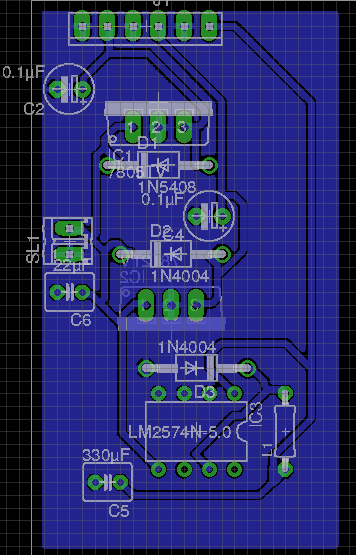
\includegraphics[angle=90,scale=0.5]{img/pcb_power.png}
\caption{PCB design of the power supply made in Eagle} 
\label{fig::pcb_power}
\end{figure}

\subsection{Color detection}
In order to detect colors a block gets shined upon with different colored LEDS.
A photo diode will give a voltage linear to the absorbed light.
This voltage will be converted to a digital signal the FPGA can work with.
In this section these modules will be described.
\subsubsection{High Power Diodes}
In order to get maximum brightness, high power diodes are used.
A diode in red, green and blue is used in order to detect different color LEGO blocks.
NTD5867NL mosfet was used to turn the diodes on and off.

The Forward voltage on the red is 1.9 V and 3.2 V for the green and blue LED\cite{ds:red_led,ds:gb_led}.
The current is chosen at $50 mA$, based on the recommended range for 100\% duty cycle\cite[p. 2]{apnote:led}.
\begin{eqnarray}
 R_{red} =& \frac{12-1.9}{0.05} =& 202 \Omega \nonumber \\
 R_{green} = R_{blue} =& \frac{12-3.2}{0.05} =& 176 \Omega \nonumber 
\end{eqnarray}
In the sorting application, the LEDs have a duty cycle of 33\% so $R_{green}$ and $R_{blue}$ is rounded down to $160 \Omega$.
The $R_{red}$ is rounded down to $200\Omega$.
The schematic can be seen in figure \ref{fig:sch_led}.
A pull down resistor at is used so the diode is not turned on without the FPGA driving it.

\begin{figure}[ht]
\centering
 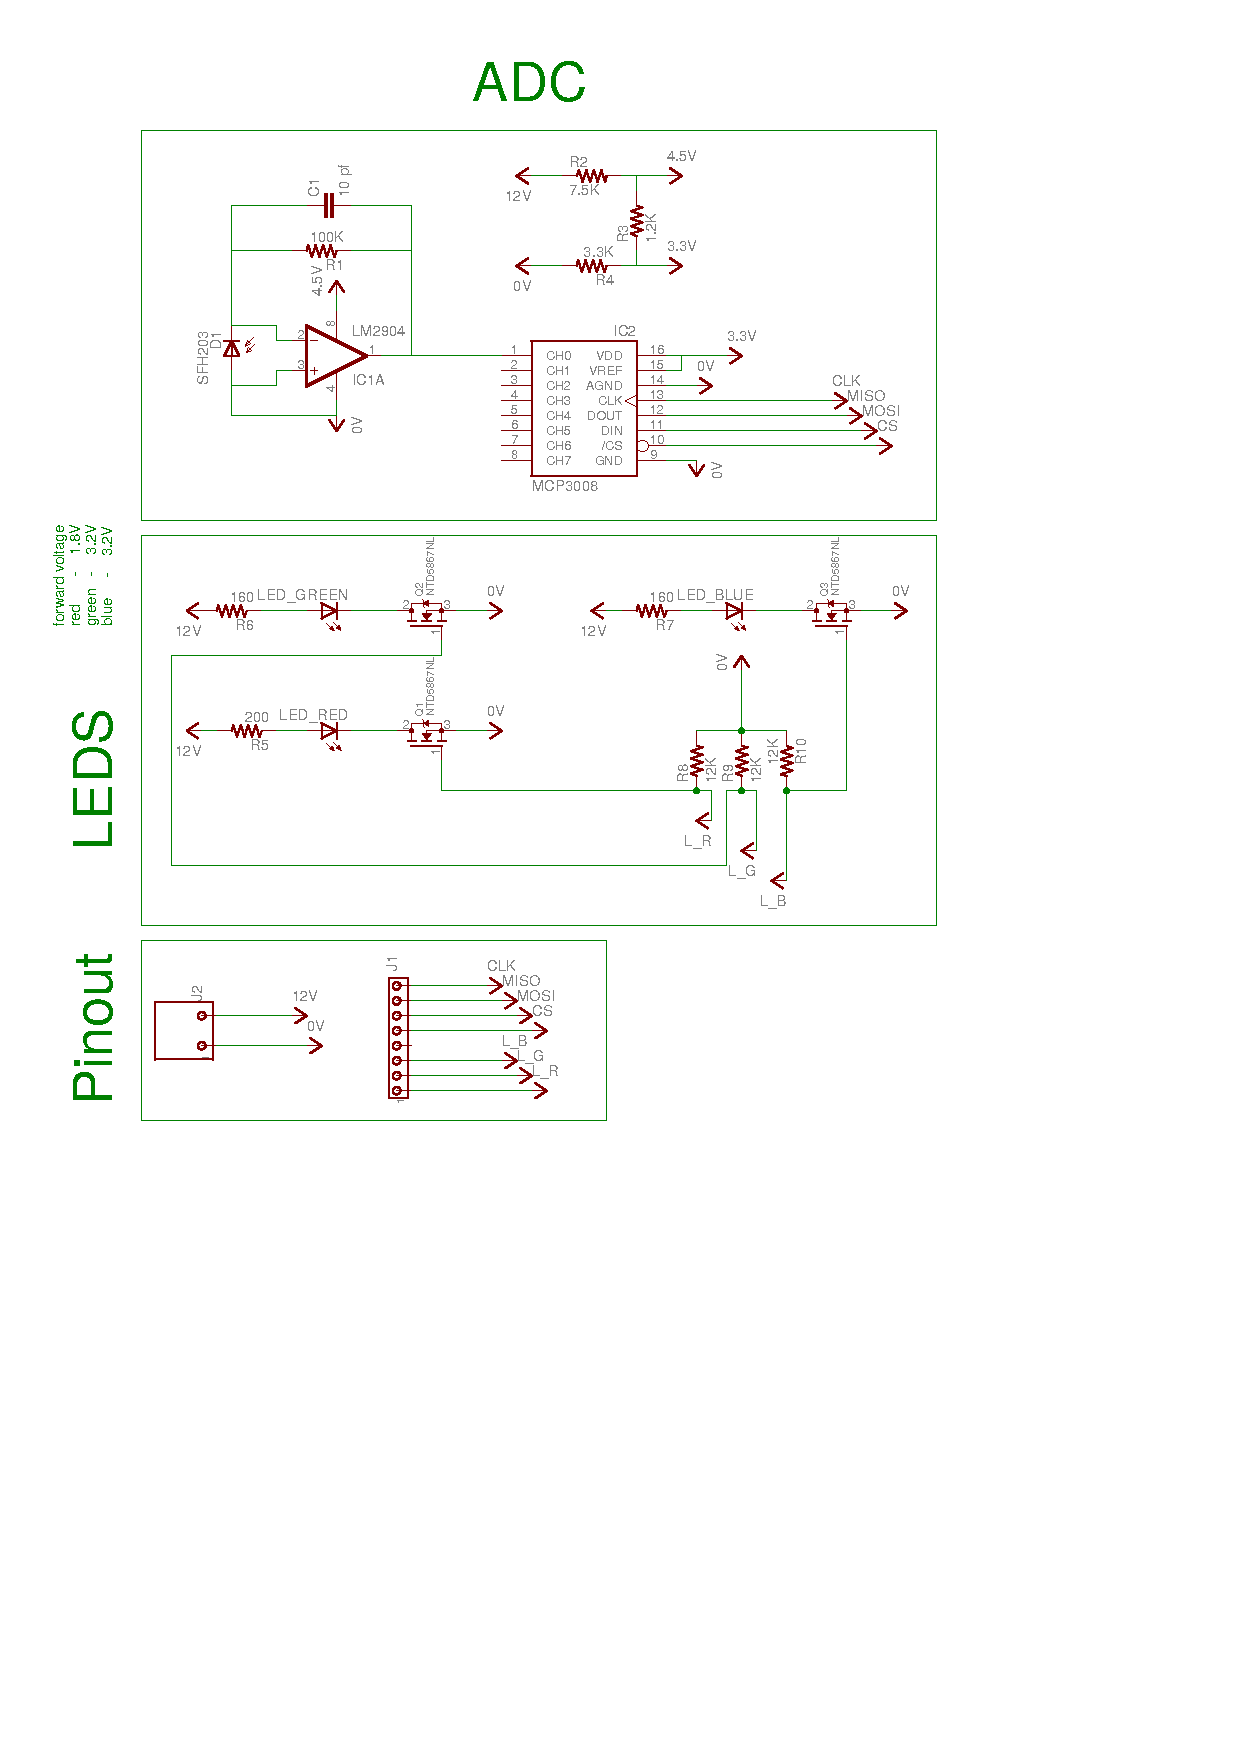
\includegraphics[scale=0.9,trim={2.4cm 14cm 5.1cm 9cm},clip]{img/adc_schematic.pdf}
  \caption{Schematic for LEDS.}
  \label{fig:sch_led}
\end{figure}

\subsubsection{Photo Diode}
The photo diode works by producing a current proportional to the light intensity it receives.
To turn this into a voltage readable by the ADC, an opamp is used.
Measurements done by holding a colored LEGO brick up to the same color light source revealed that the current, produced from the photo diode was $5-20 \mu A$.
Tests using a flashlight directly pointed at the photo diode showed that the current could get up to $40 \mu A$.
The desired output should be $0-3.3 V$, same as the logic level used on the FPGA.
If $20 \mu A$ should correlate to $2 V$, the resistor should be $100K\Omega$. 
This gives room for more intensity, so saturation of the op amp less likely with a false positive.

The LM358 is chosen for the op amp.
It can be used with a single supply, but does not have rail to rail output.
Measurements of the output shows that with a supply of 3.3 V the output can vary from 0.05 V to 2.1 V.
Thus a supply of 4.5 V is chosen so the op amp can provide an output ranging from 0.05 to 3.3 V, thus creating a pseudo rail to rail.
To get a 4.5 V supply, a voltage divider is used. This is done with 3 resistors so there is a 3.3 V supply for the ADC and a 4.5 V supply for the op amp.
The schematic for the photo diode can be seen in figure \ref{fig:sch_photo_diode}.

The MCP3001 is an ADC in a single component.
It provides a 10 bit variable, sent over SPI.
The supply is chosen to be 3.3 V, keeping the logic level the same as the FPGA.

\begin{figure}[ht]
\centering%left, bot, right, top
 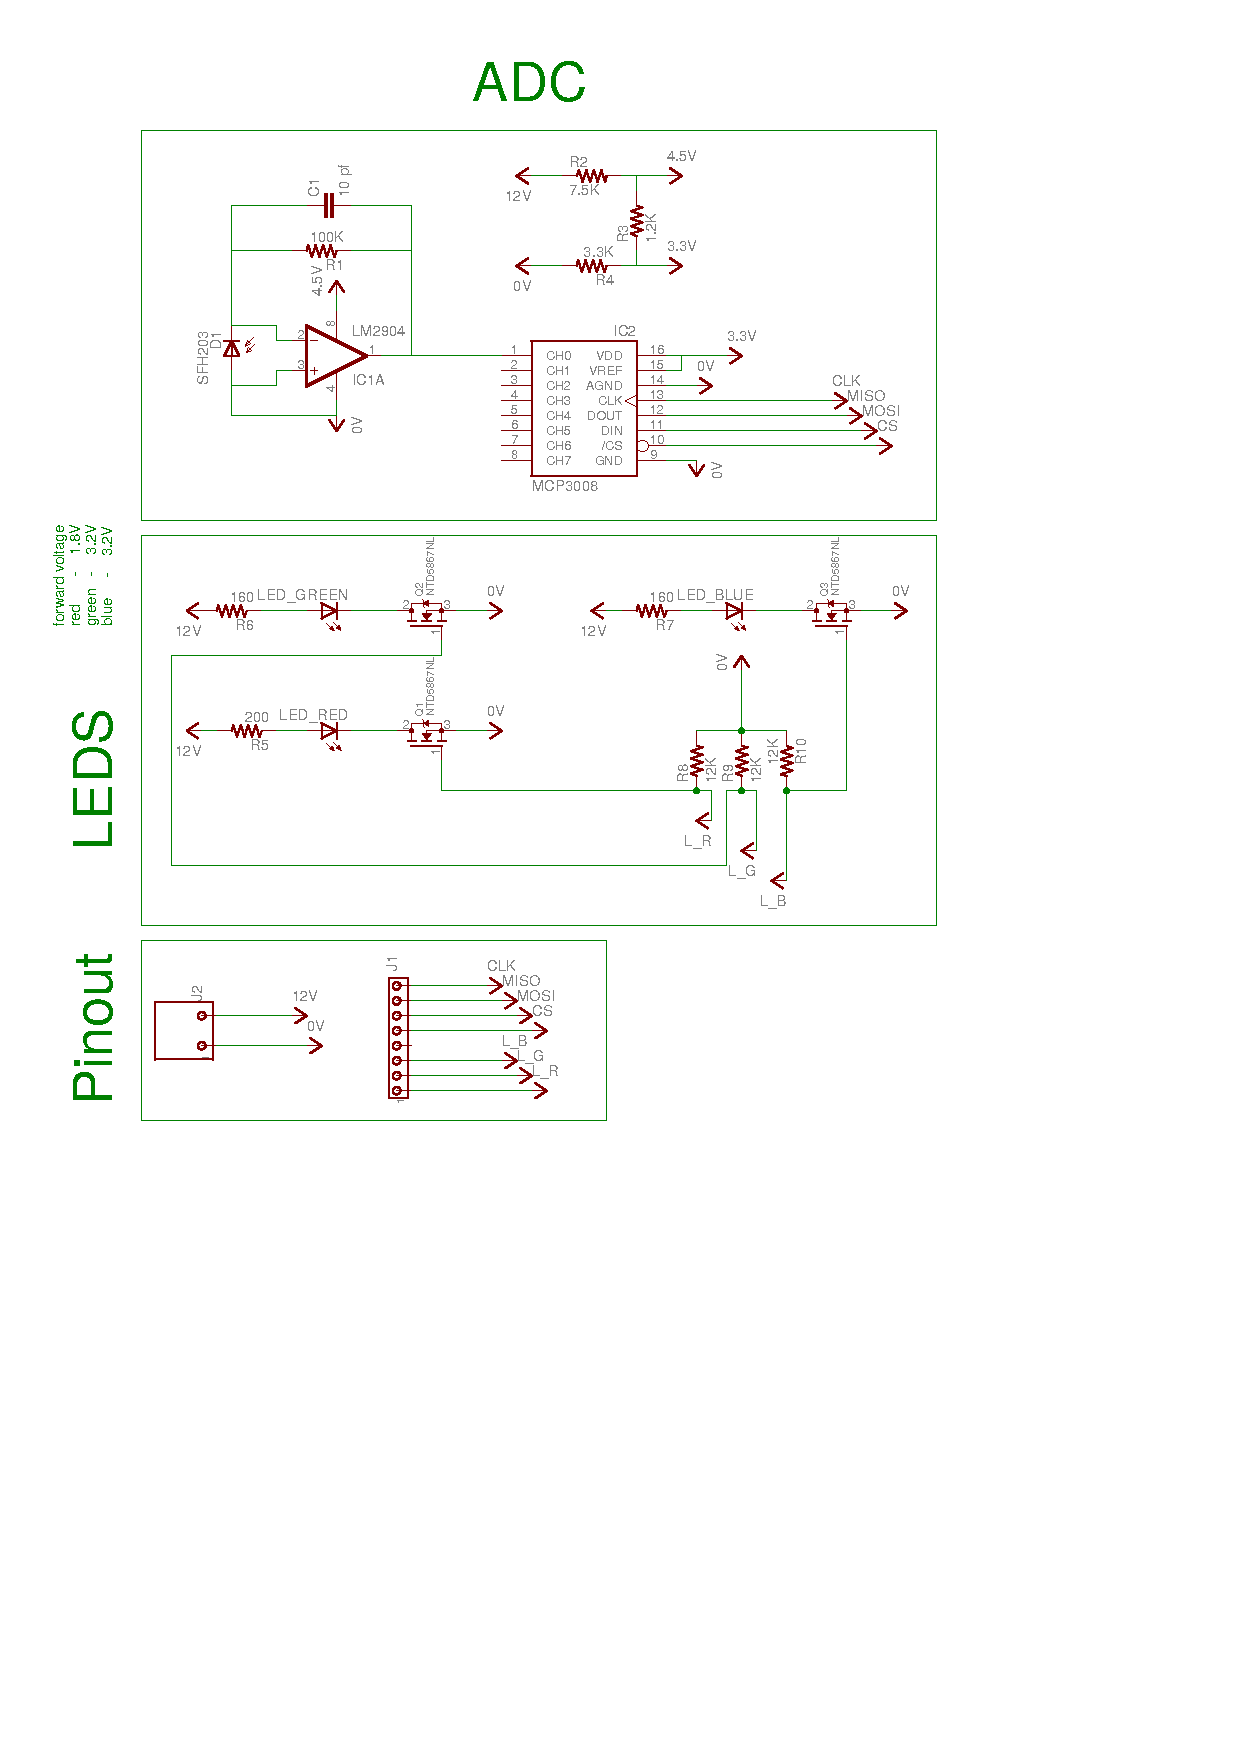
\includegraphics[scale=0.9,trim={2.4cm 20.8cm 5.1cm 2.2cm},clip]{img/adc_schematic.pdf}
  \caption{Schematic for photo diode.}
  \label{fig:sch_photo_diode}
\end{figure}

\subsubsection{PCB design}
The PCB design was made early in the process.
This means the errors in the board are still present.
Two fixes has been made to the PCB design.
The $V_+$ on the op amp has been swapped with the $V_-$.
This has been fixed by adding wires between the op-amp and the socket.
Another fix has been adding a capacitor on feedback signal to the op-amp.
This is discussed in section \ref{sec:rise_time_test}. 
The PCB can be seen in figure \ref{fig:adc_board}.

\begin{figure}[ht]                     %left, bot, right, top
\centering
 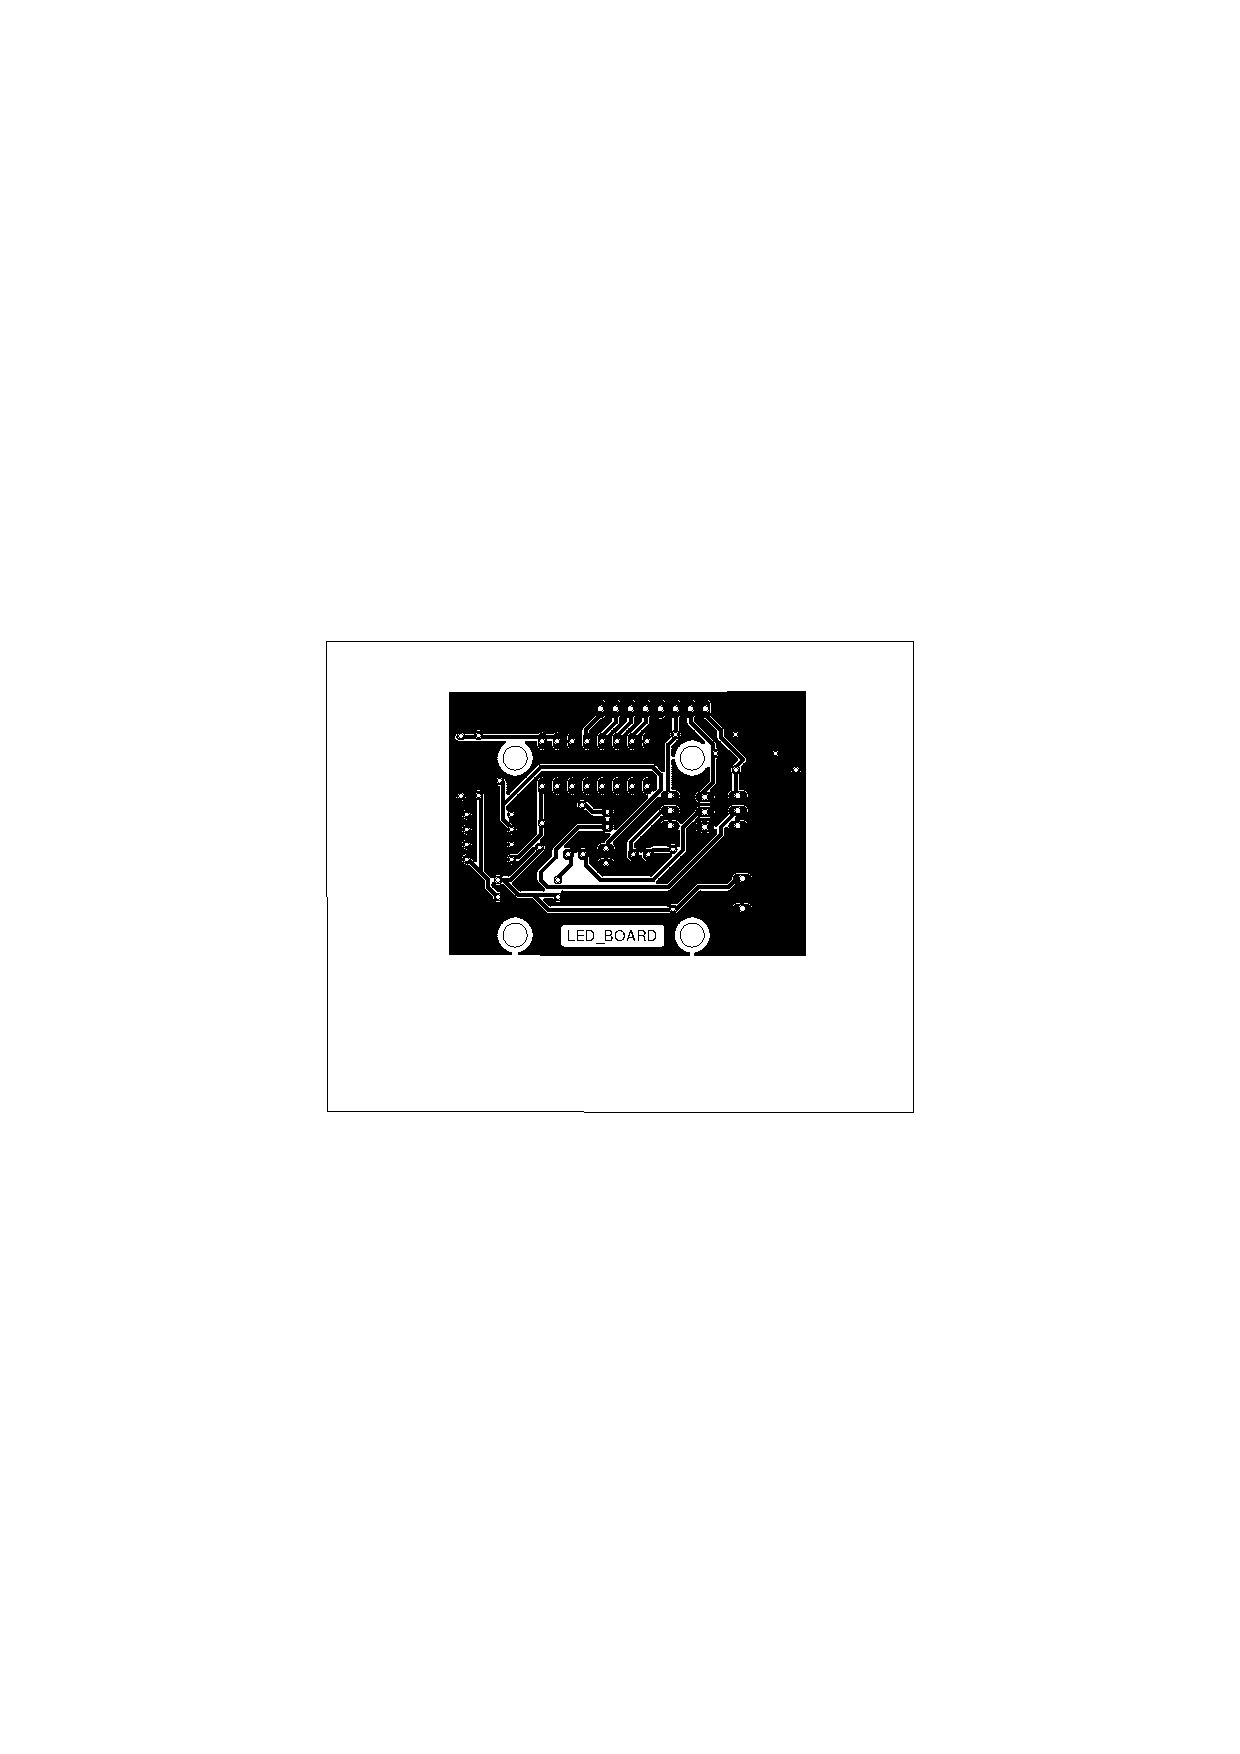
\includegraphics[scale=1,trim={7.6cm 13.5cm 8cm 11.8cm},clip]{img/printed_adc_board}
 \caption{The printed ADC board.}\label{fig:adc_board}
\end{figure}
